\documentclass[12pt]{report}

\usepackage[a4paper, margin=1in]{geometry}
\usepackage{graphicx}
\usepackage{amsmath}
\usepackage[hidelinks]{hyperref}
\usepackage{booktabs}
\usepackage{setspace}
\usepackage{svg}
\usepackage{subcaption}
\usepackage{float}

\title{Ph.D. Progress Report}
\author{Raj Singh}
\date{\today}

\begin{document}

\maketitle

% Table of Contents
\tableofcontents
\newpage

% -----------------------------

\chapter{Introduction}

\begin{spacing}{1.06}
Machine learning has emerged as a fundamental paradigm for addressing complex real-world problems across diverse domains, including healthcare, finance, and autonomous systems. In particular, advancements in computer vision have enabled machines to interpret and analyze visual data with high precision. By leveraging large-scale datasets and computational power, modern machine learning models are capable of identifying intricate patterns and relationships that are often beyond human perception. In addition to data-intensive deep learning approaches, classical machine learning methods, such as support vector machines and decision trees, remain effective, particularly in scenarios involving limited data. These methods often demonstrate robust performance on small and structured datasets, making them highly relevant in domains where large-scale data collection is challenging. Collectively, these capabilities have positioned machine learning as a key driver of innovation in data-driven scientific and industrial applications.\\

In the context of healthcare, machine learning has increasingly been adopted to support clinical decision-making and improve patient outcomes. Data-driven approaches enable the analysis of heterogeneous medical data, including clinical records, laboratory results, and patient-reported information. Such methods facilitate more objective, consistent, and scalable diagnostic processes. As a result, machine learning-based systems have the potential to reduce diagnostic errors, optimize treatment strategies, and ultimately enhance the efficiency of healthcare systems.\\

A particularly important application of machine learning in healthcare is medical image analysis. Over the past decade, approaches based on machine learning algorithms have become increasingly prominent for analyzing imaging modalities such as magnetic resonance imaging (MRI), computed tomography (CT), and X-ray scans. Recent advances in deep learning, especially convolutional neural networks, have significantly improved the ability to automatically extract hierarchical feature representations from high-dimensional image data. This enables the detection of subtle disease-specific patterns that may not be readily discernible through conventional analysis, thereby improving diagnostic accuracy, reproducibility, and scalability~\cite{litjens2017survey, esteva2017dermatologist, lecun2015deep, shen2017deep}. From a clinical perspective, faster and more accurate diagnosis can reduce healthcare costs, minimize patient burden, and alleviate both physical and psychological distress associated with delayed treatment.\\

\end{spacing}

\begin{figure}[t]
	\centering
	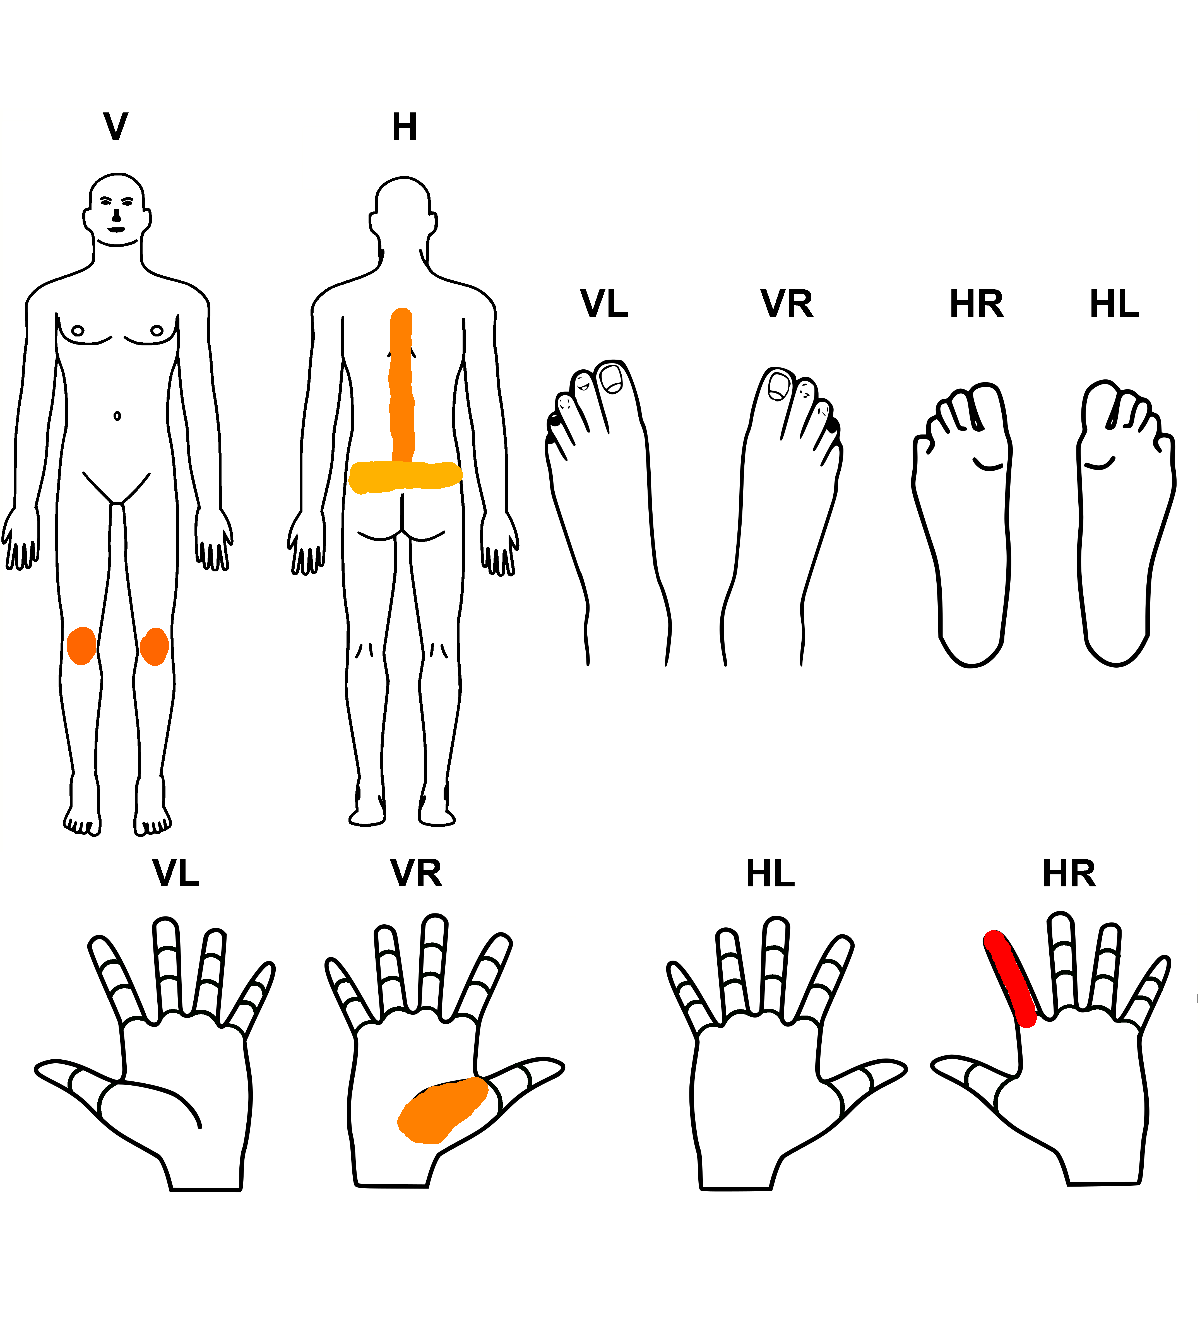
\includegraphics[width=0.5\textwidth]{pd.png}
	\caption{Pain Drawing}
	\label{fig:my_image}
\end{figure}

In addition to conventional medical imaging, alternative forms of patient-generated visual data have gained increasing attention in recent years. One such modality is pain drawings, which have been explored as a diagnostic support tool for rare and complex diseases such as Ehlers-Danlos Syndrome (EDS), Guillain-Barré Syndrome (GBS), Pompe disease, Inclusion Body Myositis (IBM), and Facioscapulohumeral Muscular Dystrophy (FSHD)~\cite{wester2020pain, emmert2018pain2d}. These conditions often exhibit heterogeneous and overlapping symptom patterns, making accurate diagnosis challenging using traditional clinical approaches. The integration of machine learning techniques with pain drawing data provides an opportunity to analyze spatial pain patterns in a systematic and quantitative manner, thereby supporting disease classification and improving diagnostic reliability.\\

Pain drawings (PDs) are structured visual representations in which patients indicate the spatial distribution of perceived pain on a standardized human body template. These templates typically include multiple anatomical perspectives, such as anterior, posterior, and lateral views, along with detailed representations of extremities including hands and feet. Pain drawings can be generated using traditional paper-based methods or digital platforms, enabling consistent and scalable data acquisition. The spatial information encoded in pain drawings serves as a valuable source of discriminative features, which can be leveraged by computational models for both binary and multi-class classification tasks. Prior studies have demonstrated that such approaches, including systems like Pain2D, can effectively utilize pain drawings to enhance diagnostic performance and support clinical decision-making~\cite{wester2020pain, emmert2018pain2d}.


\chapter{Related Works}


% -----------------------------
\chapter{Dataset Acquisition and Description}

\section{Conventional Pain Drawing Collection}

In prior studies, pain drawings were primarily collected using traditional analytical methods, where patients marked perceived pain regions on a printed human body outline. These paper-based representations were subsequently digitized through scanning, enabling the application of computational algorithms for further analysis. While this approach provides a structured means of capturing spatial pain information, it introduces several inherent limitations.\\

One significant challenge arises from the scanning process itself, which often leads to alignment inconsistencies across samples. Variations in scale, orientation, and positioning of the scanned images can negatively impact downstream analysis, particularly in machine learning pipelines that rely on spatial consistency. Additionally, conventional pain drawings typically capture only the location of pain, without providing any quantitative representation of pain intensity. As a result, valuable information regarding the severity of symptoms is lost, limiting the expressiveness and diagnostic utility of the dataset.\\


To address the aforementioned limitations, a digital approach for pain data acquisition is required. In particular, eliminating the need for scanning can ensure consistent alignment and standardization across all samples. Furthermore, incorporating mechanisms to capture pain intensity, in addition to spatial location, can significantly enhance the richness of the dataset. Such improvements are essential for enabling more robust and informative machine learning-based analysis.\\


To overcome the challenges associated with traditional data collection, a dedicated application, referred to as \textit{SeePain}, was developed. The application provides a digital interface that allows patients to directly annotate pain regions on a standardized human body template. By design, this approach ensures consistent alignment across all collected samples, thereby eliminating preprocessing challenges related to image registration and normalization.\\

In addition to capturing the spatial distribution of pain, the SeePain application incorporates functionality to represent pain intensity. This is achieved through a controlled color-coding mechanism, enabling patients to indicate varying levels of pain severity. Consequently, the collected data contains both spatial and intensity information, which enhances its suitability for downstream machine learning tasks.

\section{Seepain}
Yet, to be written...

\section{Datasets Description}

\begin{table}[h]
	\centering
	\begin{tabular}{|l|l|c|c|}
		\hline
		\textbf{Dataset Source} & \textbf{Classes} & \textbf{Samples per Class} & \textbf{Total Samples} \\
		\hline
		RWTH Aachen University & Others & 59 & \\
		& gHSD & 45 & \\
		& hEDS & 141 & 245 \\
		\hline
		MHH (IDANA Application) & Arthritis & 69 & \\
		& Kollagenose & 22 & \\
		& Polyarthritis & 359 & \\
		& Polymyalgia & 65 & \\
		& Sjögren Syndrome & 38 & \\
		& Spondyloarthritis & 147 & \\
		& Unknown & 185 & 885 \\
		\hline
		MHH (SeePain Application) & Myositis & 4 & \\
		& Polymyalgia rheumatica & 7 & \\
		& Psoriasis-Arthritis & 17 & \\
		& Rheumatoide Arthritis & 35 & \\
		& Riesenzellarteriitis & 1 & \\
		& Sonstige & 31 & \\
		& axiale Spondyloarthritis & 10 & \\
		& nan & 7 & 124 \\
		\hline
		Munich Dataset & FSHD & 34 & \\
		& POMPE & 76 & \\
		& IBM & 16 & \\
		& SMA & 22 & 148 \\
		\hline
	\end{tabular}
	\caption{Overview of datasets, class distribution, and total number of samples. Both the IDANA and SeePain datasets originate from Hannover Medical School (MHH).}
	\label{tab:dataset_overview}
\end{table}

A total of three medical institutions contributed datasets to this study, namely Hannover Medical School (MHH), RWTH Aachen University, and a medical institution in Munich. From MHH, data were collected using two different applications, namely the IDANA application and the SeePain application, resulting in two distinct datasets.\\

The dataset obtained from RWTH Aachen University comprises three classes: Others, generalized hypermobility spectrum disorder (gHSD), and hypermobile Ehlers-Danlos syndrome (hEDS), with 59, 45, and 141 samples, respectively.\\

The IDANA dataset collected at MHH is more diverse and consists of seven diagnostic categories: Arthritis, Kollagenose, Polyarthritis, Polymyalgia, Sjögren Syndrome, Spondyloarthritis, and Unknown, containing 69, 22, 359, 65, 38, 147, and 185 samples in each class, respectively.\\

In addition, the dataset collected using the SeePain application at MHH comprises 124 samples distributed across eight classes: Myositis (4 samples), Polymyalgia rheumatica (7), Psoriasis-Arthritis (17), Rheumatoide Arthritis (35), Riesenzellarteriitis (1), Sonstige (31), axiale Spondyloarthritis (10), and nan (7). This fine-grained class annotation enables a more detailed analysis of patient-reported pain patterns.\\

Finally, the dataset obtained from Munich comprises four classes: Facioscapulohumeral Muscular Dystrophy (FSHD), Pompe disease, Inclusion Body Myositis (IBM), and Spinal Muscular Atrophy (SMA), consisting of 34, 76, 16, and 22 samples, respectively. Overall, these datasets exhibit considerable variability in terms of class distribution, dataset size, and acquisition methodology, which introduces challenges such as class imbalance and domain heterogeneity for subsequent machine learning-based analysis.





% -----------------------------
\chapter{Methodology and Pipeline}

\section{Overview}

This chapter describes the overall pipeline employed in this study, encompassing data loading, preprocessing, model development, training, and evaluation. The objective of this pipeline is to ensure a systematic and reproducible framework for analyzing pain drawing datasets using machine learning techniques.

\section{Data Loading}

In the initial stage, datasets obtained from multiple sources are loaded into the computational environment. This includes data from RWTH Aachen University, Hannover Medical School (MHH) through the IDANA and SeePain applications, and the Munich dataset. Each dataset is organized according to its respective class labels and prepared for further processing.

\section{Data Preprocessing}

To ensure consistency across datasets and improve model performance, several preprocessing steps are applied. These include:

\begin{itemize}
	\item \textbf{Resizing:} All images are resized to a uniform spatial resolution to maintain consistency across samples.
	\item \textbf{Grayscale Conversion:} RGB images are converted to grayscale to reduce computational complexity and focus on structural information.
	\item \textbf{Thresholding:} Thresholding techniques are applied to enhance relevant regions and suppress noise.
\end{itemize}

\section{Model Development}

Four different neural network architectures are designed and evaluated in this study:

\begin{itemize}
	\item \textbf{Small Convolutional Neural Network (CNN)}
	\item \textbf{Large Convolutional Neural Network (CNN)}
	\item \textbf{Small Fully Connected Neural Network (FCNN)}
	\item \textbf{Large Fully Connected Neural Network (FCNN)}
\end{itemize}

These models are developed to analyze the impact of architectural complexity on classification performance.

\section{Training Setup}

All models are trained using a consistent set of hyperparameters to ensure fair comparison. The training configuration is as follows:

\begin{itemize}
	\item \textbf{Number of Epochs:} 50
	\item \textbf{Learning Rate:} 0.001
	\item \textbf{Batch Size:} 16
	\item \textbf{Training Split:} 90\% of the data is used for training, while the remaining 10\% is reserved for validation.
\end{itemize}

\section{Evaluation Metrics}

The performance of the models is evaluated using standard metrics, including:

\begin{itemize}
	\item \textbf{Training Loss}
	\item \textbf{Training Accuracy}
	\item \textbf{Validation Loss}
	\item \textbf{Validation Accuracy}
\end{itemize}

These metrics provide insights into model convergence, generalization capability, and potential overfitting during training.

% -----------------------------
\chapter{Experiments}

% -----------------------------
\chapter{Results}
\begin{figure}[H]
	\centering
	
	% ================= Row 1: Model 1 =================
	\begin{subfigure}{0.3\textwidth}
		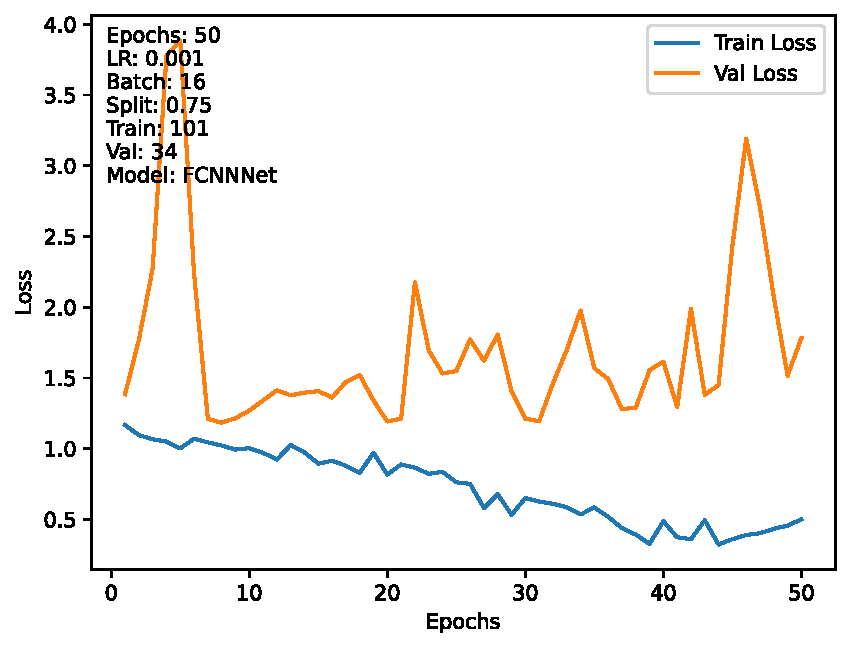
\includegraphics[width=\linewidth]{images/aachen_num_classes_3_FCNNNet_loss.pdf}
		\caption{FCNNNet - Loss}
	\end{subfigure}
	\hfill
	\begin{subfigure}{0.3\textwidth}
		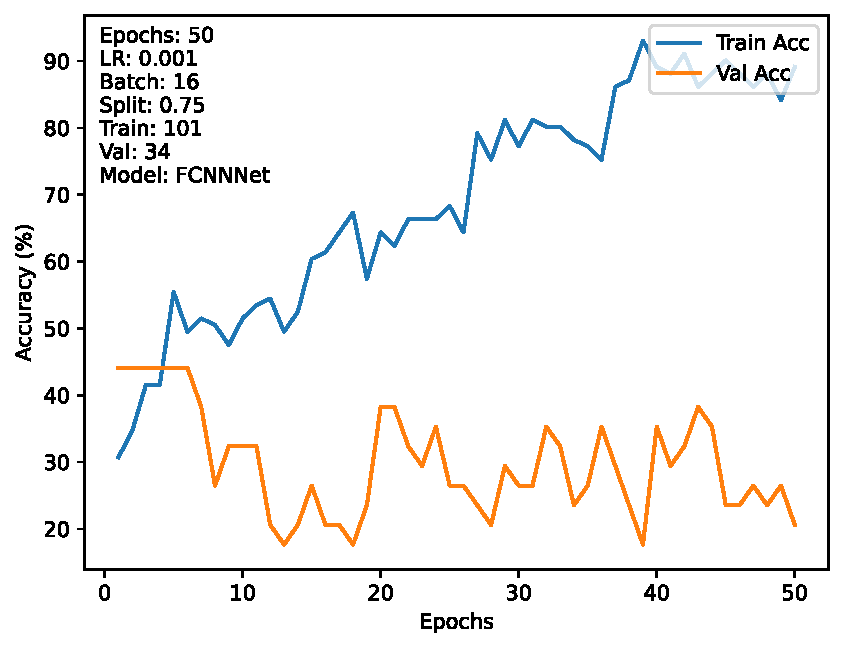
\includegraphics[width=\linewidth]{images/aachen_num_classes_3_FCNNNet_accuracy.pdf}
		\caption{FCNNNet - Accuracy}
	\end{subfigure}
	\hfill
	\begin{subfigure}{0.3\textwidth}
		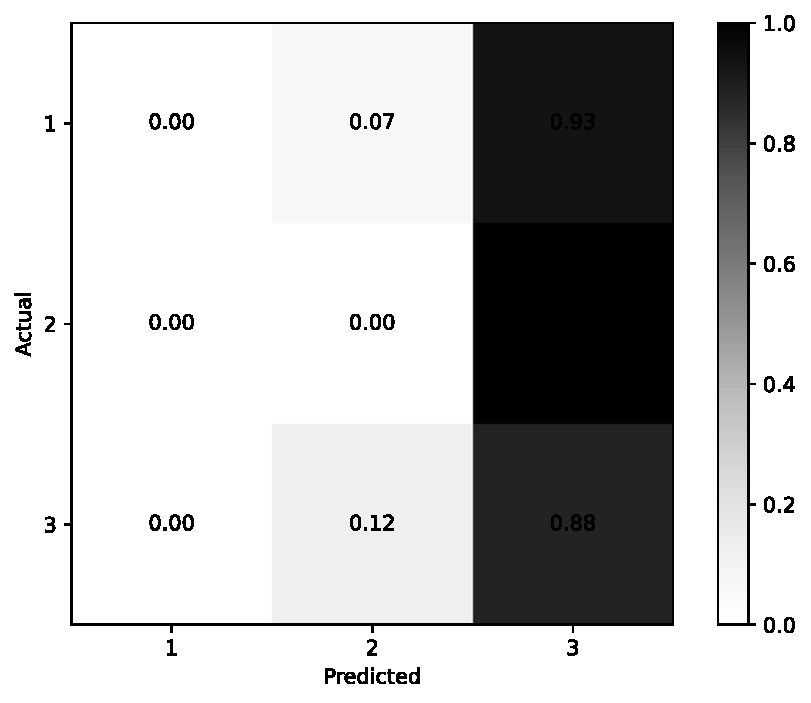
\includegraphics[width=\linewidth]{images/aachen_num_classes_3_FCNNNet_confusion_matrix.pdf}
		\caption{FCNNNet - Confusion Matrix}
	\end{subfigure}
	
	\vspace{0.3cm}
	
	% ================= Row 2: Model 2 =================
	\begin{subfigure}{0.3\textwidth}
		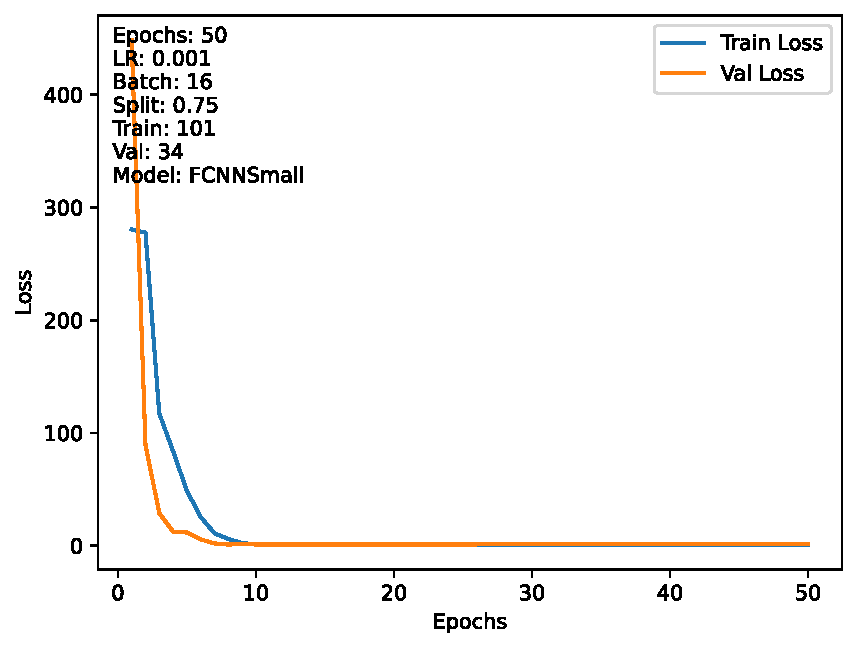
\includegraphics[width=\linewidth]{images/aachen_num_classes_3_FCNNSmall_loss.pdf}
		\caption{FCNNSmall - Loss}
	\end{subfigure}
	\hfill
	\begin{subfigure}{0.3\textwidth}
		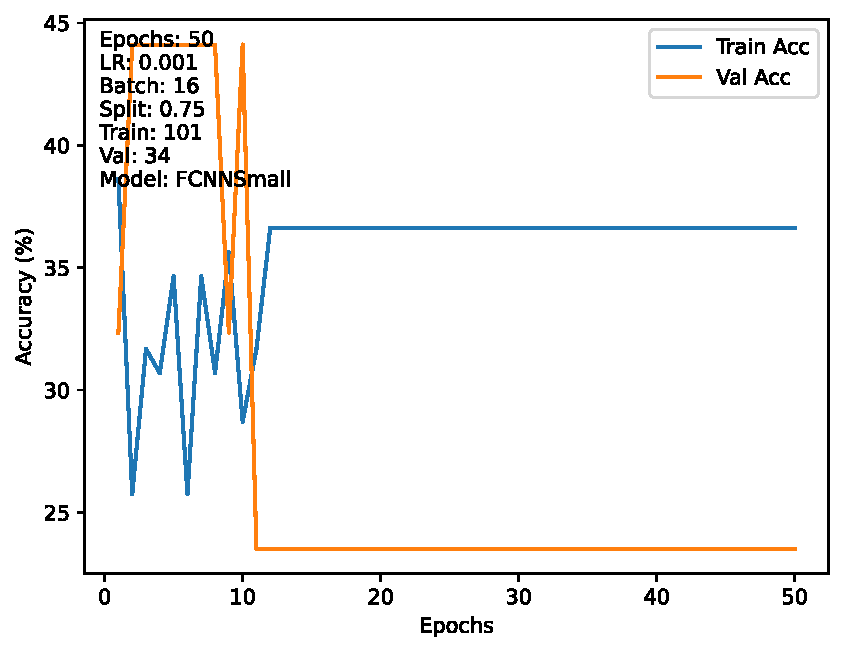
\includegraphics[width=\linewidth]{images/aachen_num_classes_3_FCNNSmall_accuracy.pdf}
		\caption{FCNNSmall - Accuracy}
	\end{subfigure}
	\hfill
	\begin{subfigure}{0.3\textwidth}
		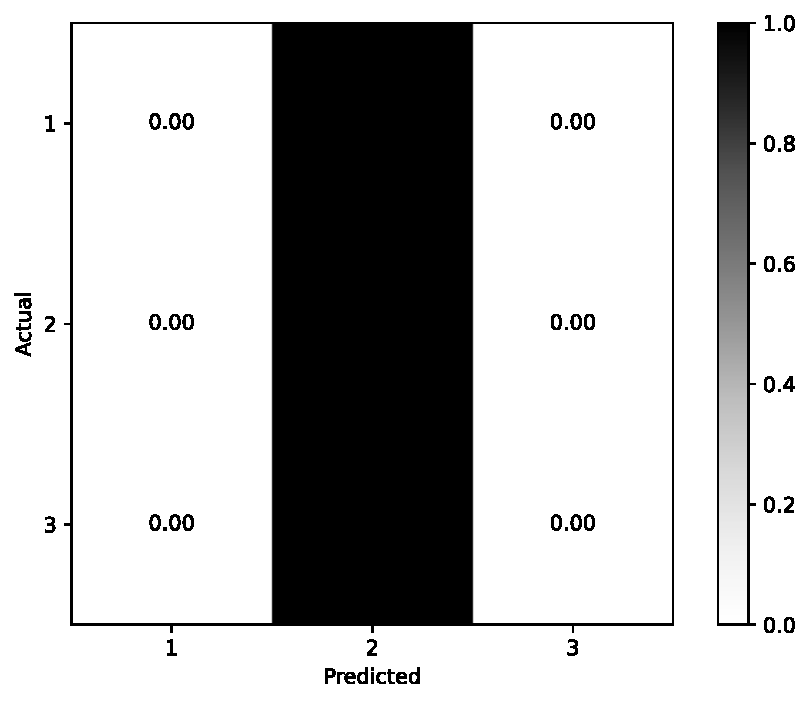
\includegraphics[width=\linewidth]{images/aachen_num_classes_3_FCNNSmall_confusion_matrix.pdf}
		\caption{FCNNSmall - Confusion Matrix}
	\end{subfigure}
	
	\vspace{0.3cm}
	
	% ================= Row 3: Model 3 =================
	\begin{subfigure}{0.3\textwidth}
		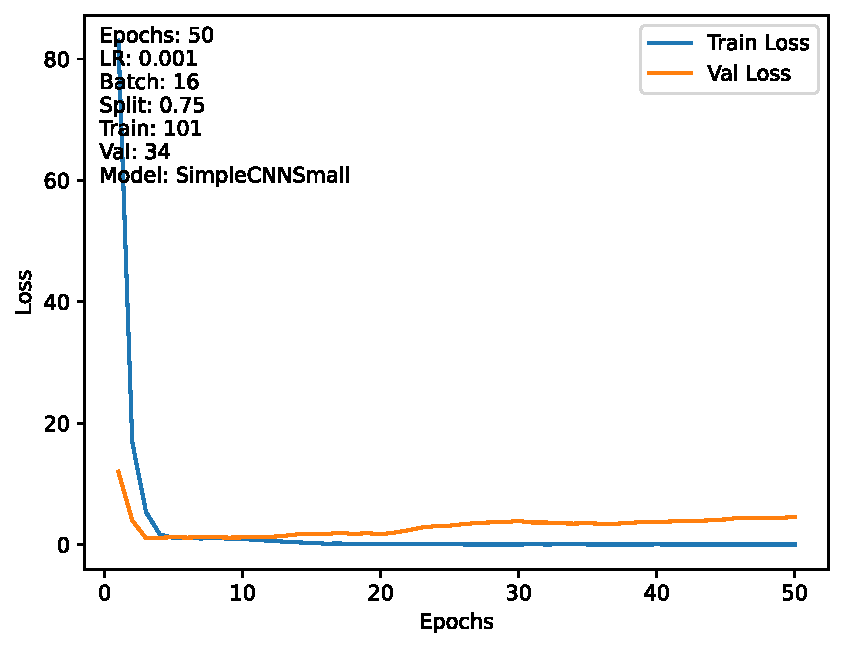
\includegraphics[width=\linewidth]{images/aachen_num_classes_3_SimpleCNNSmall_loss.pdf}
		\caption{SimpleCNNSmall - Loss}
	\end{subfigure}
	\hfill
	\begin{subfigure}{0.3\textwidth}
		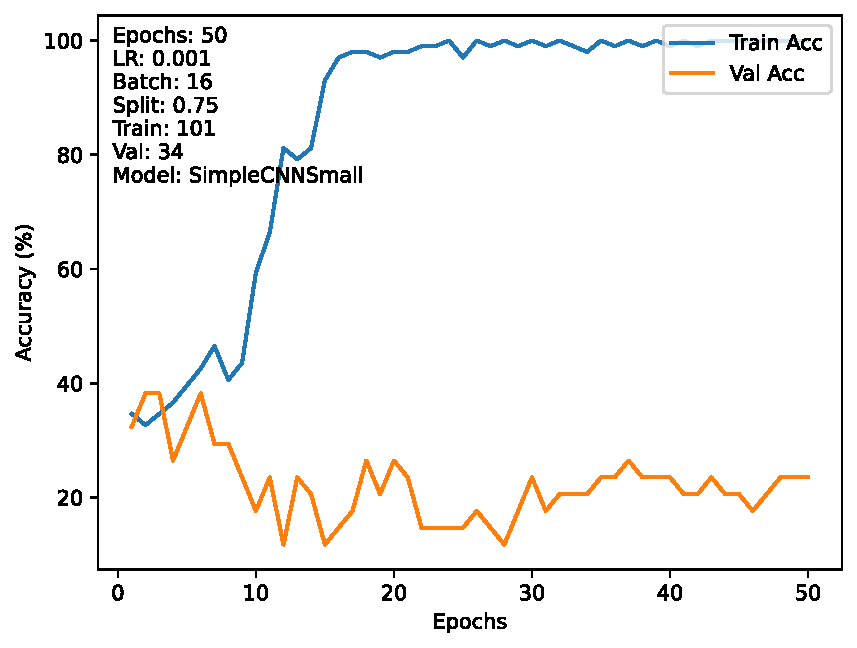
\includegraphics[width=\linewidth]{images/aachen_num_classes_3_SimpleCNNSmall_accuracy.pdf}
		\caption{SimpleCNNSmall - Accuracy}
	\end{subfigure}
	\hfill
	\begin{subfigure}{0.3\textwidth}
		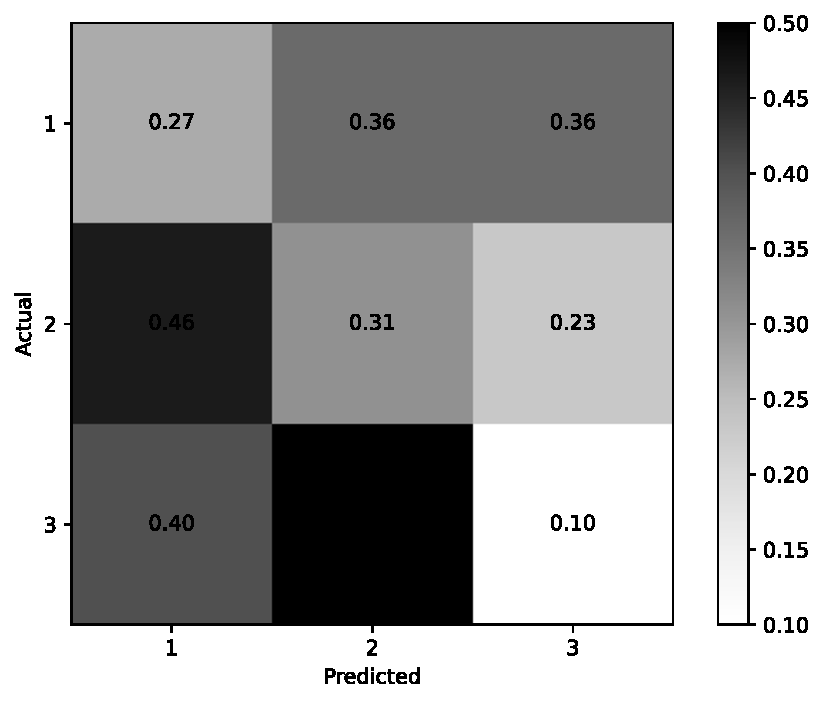
\includegraphics[width=\linewidth]{images/aachen_num_classes_3_SimpleCNNSmall_confusion_matrix.pdf}
		\caption{SimpleCNNSmall - Confusion Matrix}
	\end{subfigure}
	
	\caption{Dataset 1: Model comparison (Loss, Accuracy, and Confusion Matrix) — Aachen dataset}
\end{figure}
\newpage

\begin{figure}[H]
	\centering
	
	% ================= Row 1: Model 1 =================
	\begin{subfigure}{0.3\textwidth}
		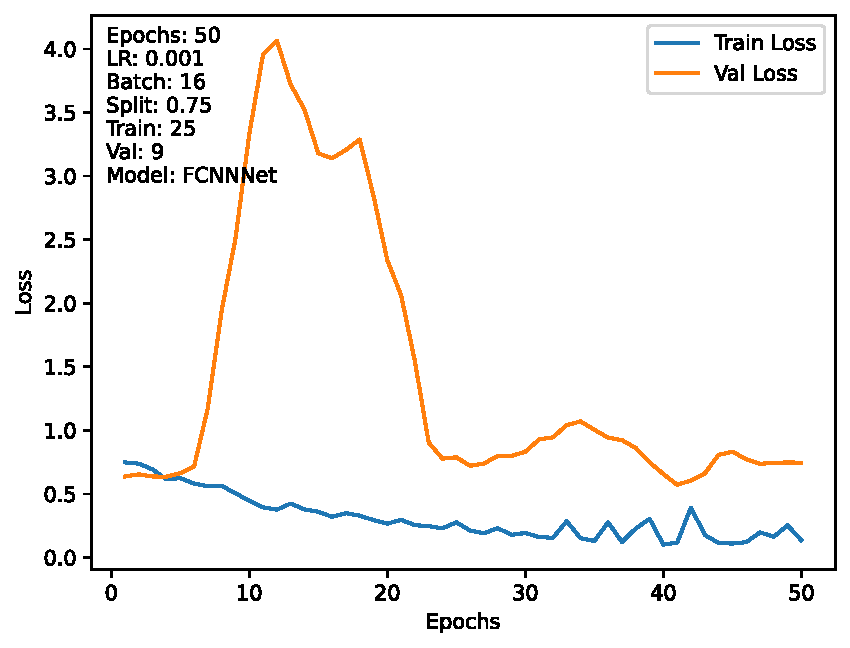
\includegraphics[width=\linewidth]{images/mhh_seepain_num_classes_2_FCNNNet_loss.pdf}
		\caption{FCNNNet - Loss}
	\end{subfigure}
	\hfill
	\begin{subfigure}{0.3\textwidth}
		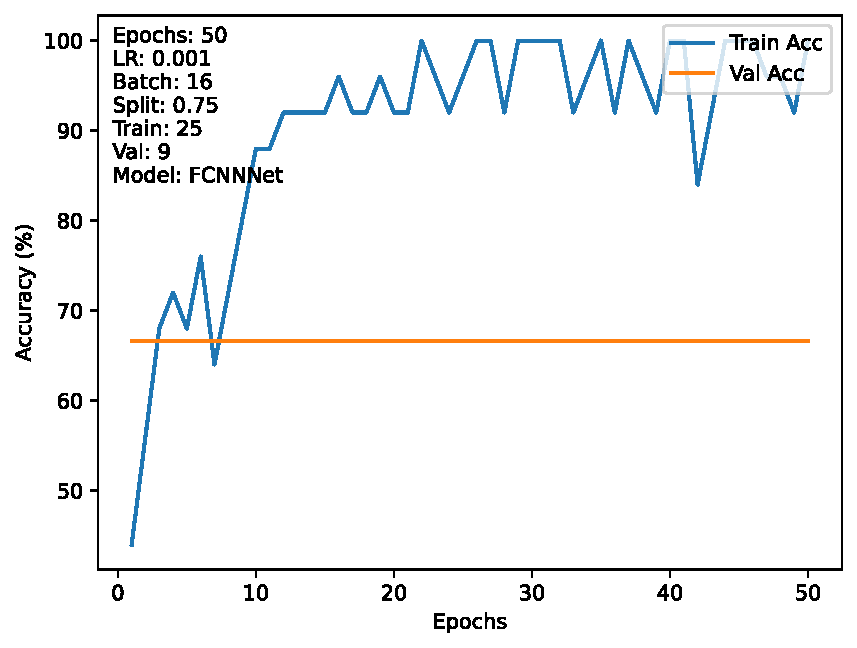
\includegraphics[width=\linewidth]{images/mhh_seepain_num_classes_2_FCNNNet_accuracy.pdf}
		\caption{FCNNNet - Accuracy}
	\end{subfigure}
	\hfill
	\begin{subfigure}{0.3\textwidth}
		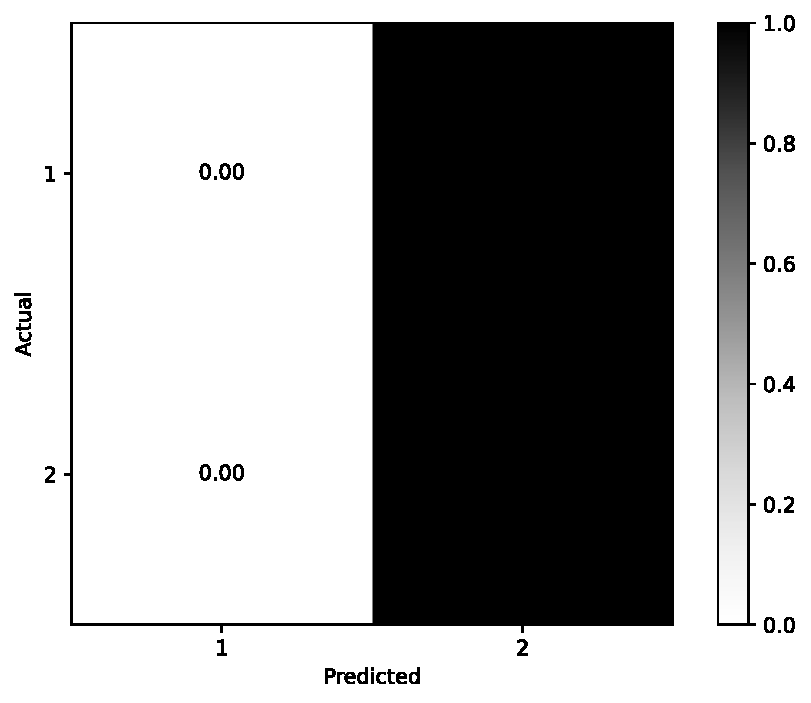
\includegraphics[width=\linewidth]{images/mhh_seepain_num_classes_2_FCNNNet_confusion_matrix.pdf}
		\caption{FCNNNet - Confusion Matrix}
	\end{subfigure}
	
	\vspace{0.3cm}
	
	% ================= Row 2: Model 2 =================
	\begin{subfigure}{0.3\textwidth}
		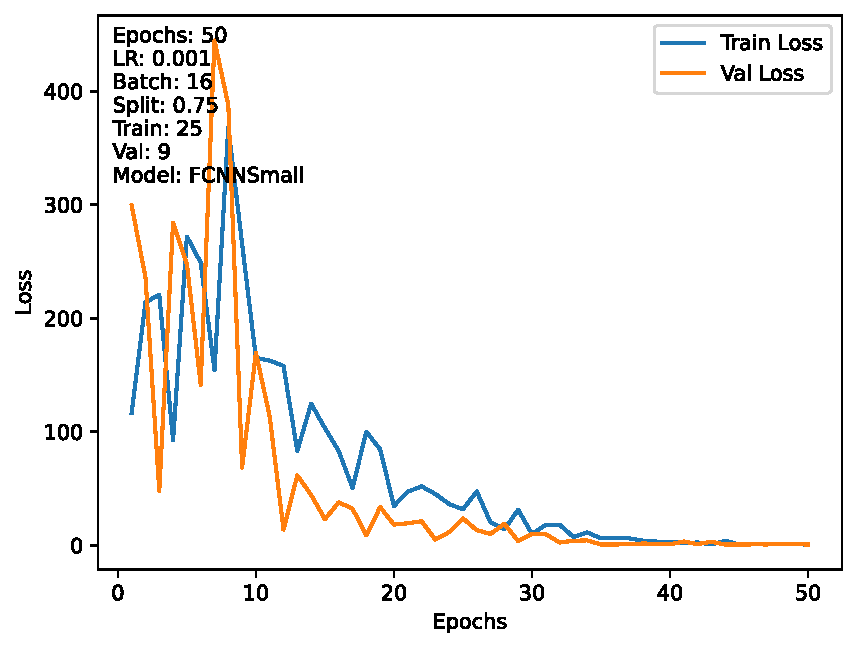
\includegraphics[width=\linewidth]{images/mhh_seepain_num_classes_2_FCNNSmall_loss.pdf}
		\caption{FCNNSmall - Loss}
	\end{subfigure}
	\hfill
	\begin{subfigure}{0.3\textwidth}
		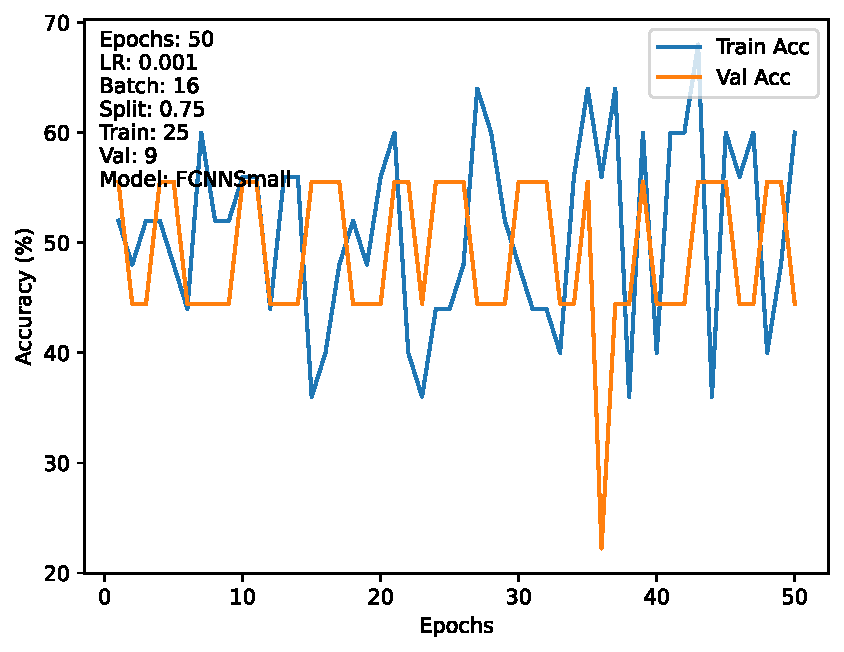
\includegraphics[width=\linewidth]{images/mhh_seepain_num_classes_2_FCNNSmall_accuracy.pdf}
		\caption{FCNNSmall - Accuracy}
	\end{subfigure}
	\hfill
	\begin{subfigure}{0.3\textwidth}
		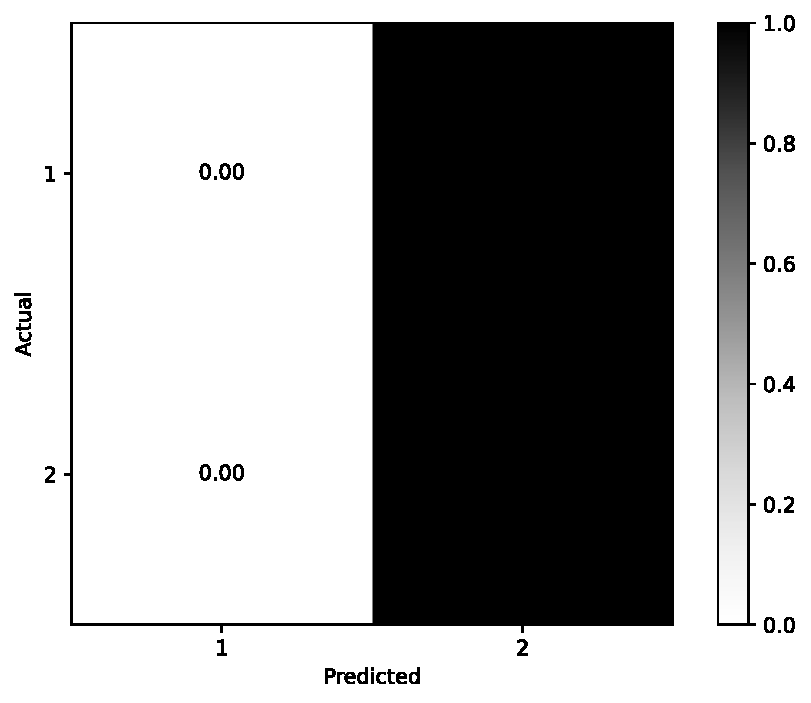
\includegraphics[width=\linewidth]{images/mhh_seepain_num_classes_2_FCNNSmall_confusion_matrix.pdf}
		\caption{FCNNSmall - Confusion Matrix}
	\end{subfigure}
	
	\vspace{0.3cm}
	
	% ================= Row 3: Model 3 =================
	\begin{subfigure}{0.3\textwidth}
		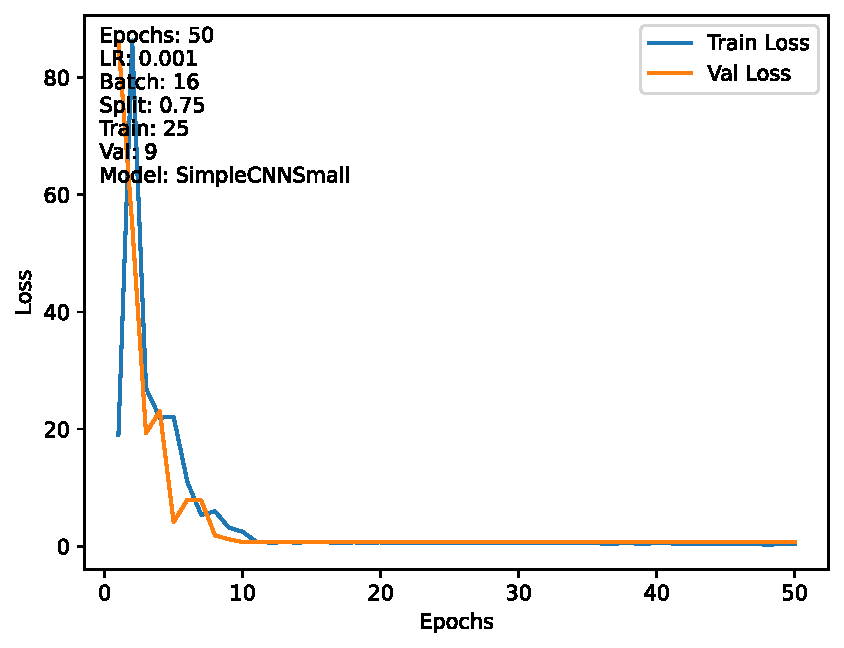
\includegraphics[width=\linewidth]{images/mhh_seepain_num_classes_2_SimpleCNNSmall_loss.pdf}
		\caption{SimpleCNNSmall - Loss}
	\end{subfigure}
	\hfill
	\begin{subfigure}{0.3\textwidth}
		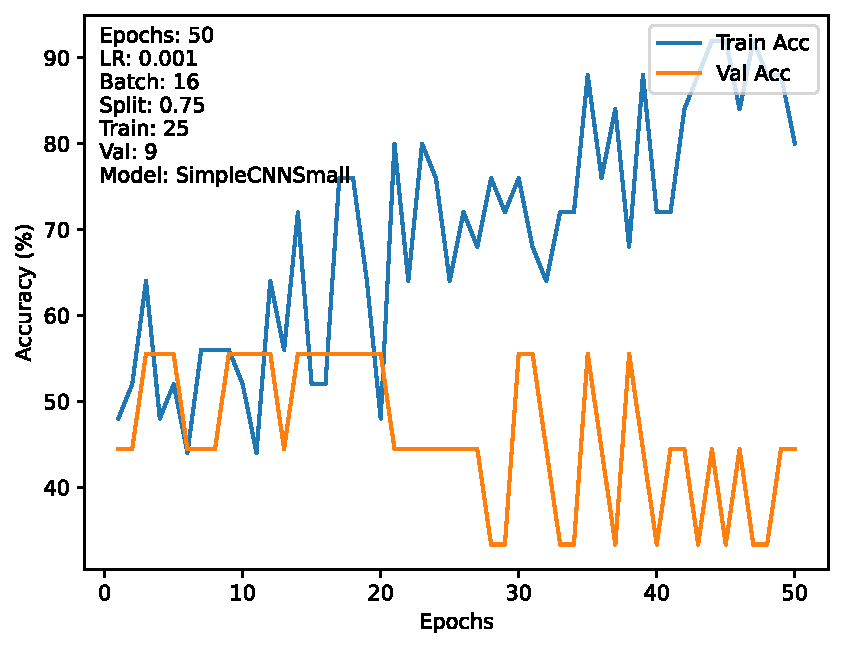
\includegraphics[width=\linewidth]{images/mhh_seepain_num_classes_2_SimpleCNNSmall_accuracy.pdf}
		\caption{SimpleCNNSmall - Accuracy}
	\end{subfigure}
	\hfill
	\begin{subfigure}{0.3\textwidth}
		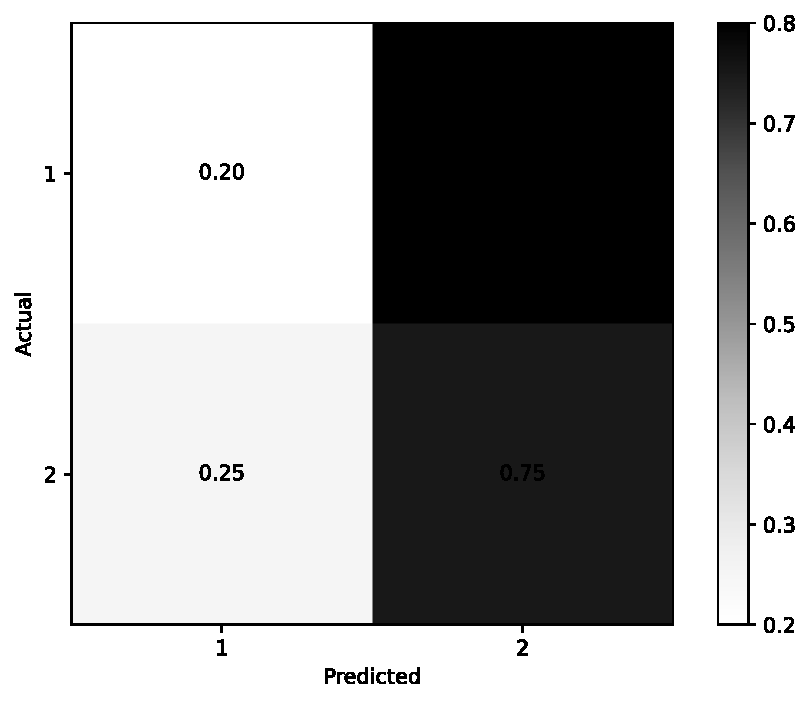
\includegraphics[width=\linewidth]{images/mhh_seepain_num_classes_2_SimpleCNNSmall_confusion_matrix.pdf}
		\caption{SimpleCNNSmall - Confusion Matrix}
	\end{subfigure}
	
	\caption{Dataset 2: Model comparison (Loss, Accuracy, and Confusion Matrix) — MHH SeePain dataset, 2 classes}
\end{figure}

\newpage

\begin{figure}[H]
	\centering
	
	% ================= Row 1: Model 1 =================
	\begin{subfigure}{0.3\textwidth}
		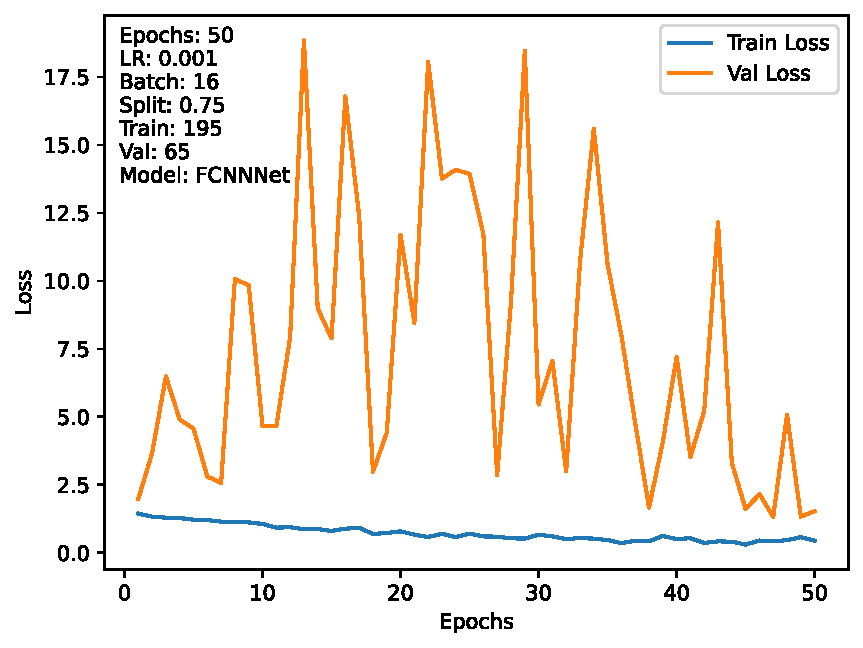
\includegraphics[width=\linewidth]{images/mhh_idana_num_classes_4_FCNNNet_loss.pdf}
		\caption{FCNNNet - Loss}
	\end{subfigure}
	\hfill
	\begin{subfigure}{0.3\textwidth}
		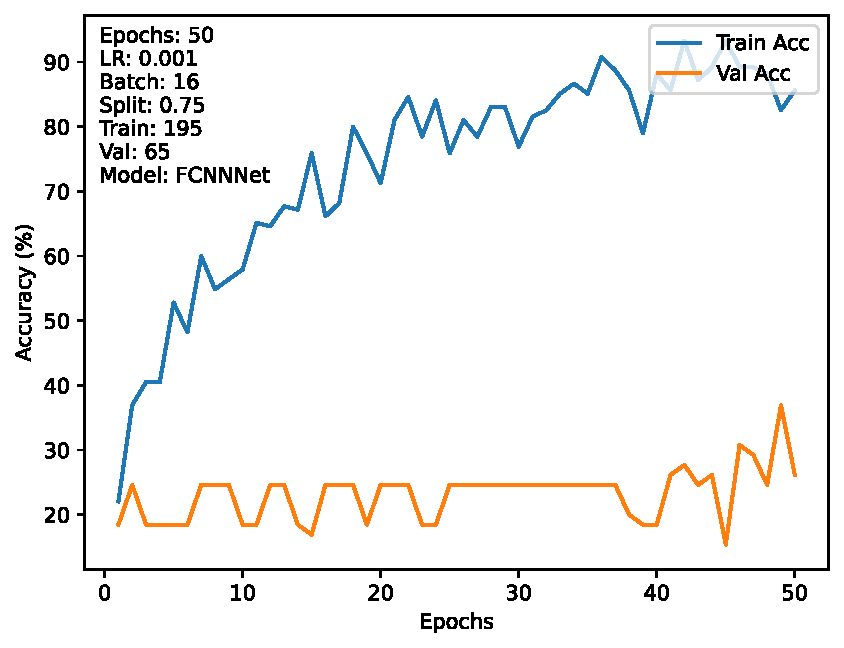
\includegraphics[width=\linewidth]{images/mhh_idana_num_classes_4_FCNNNet_accuracy.pdf}
		\caption{FCNNNet - Accuracy}
	\end{subfigure}
	\hfill
	\begin{subfigure}{0.3\textwidth}
		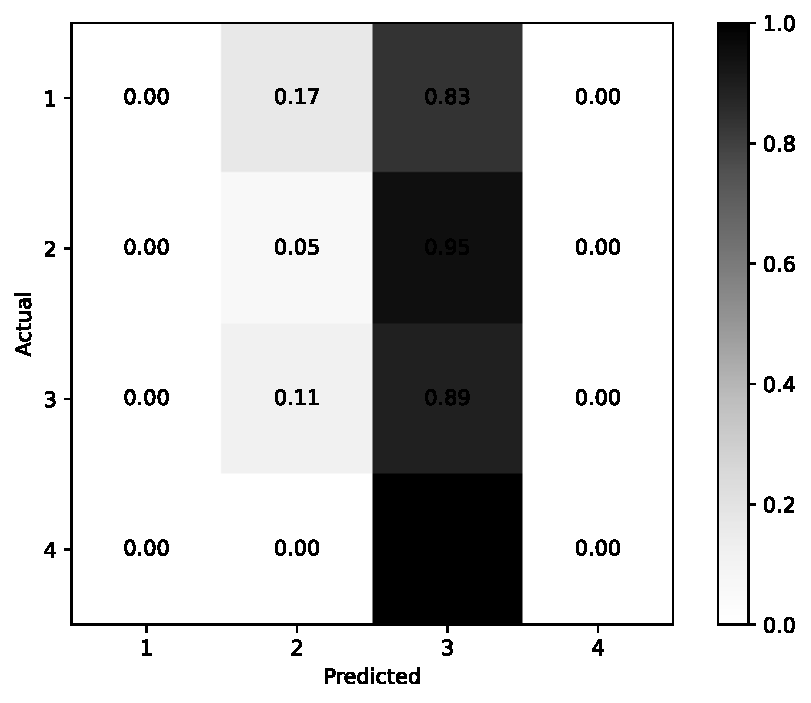
\includegraphics[width=\linewidth]{images/mhh_idana_num_classes_4_FCNNNet_confusion_matrix.pdf}
		\caption{FCNNNet - Confusion Matrix}
	\end{subfigure}
	
	\vspace{0.3cm}
	
	% ================= Row 2: Model 2 =================
	\begin{subfigure}{0.3\textwidth}
		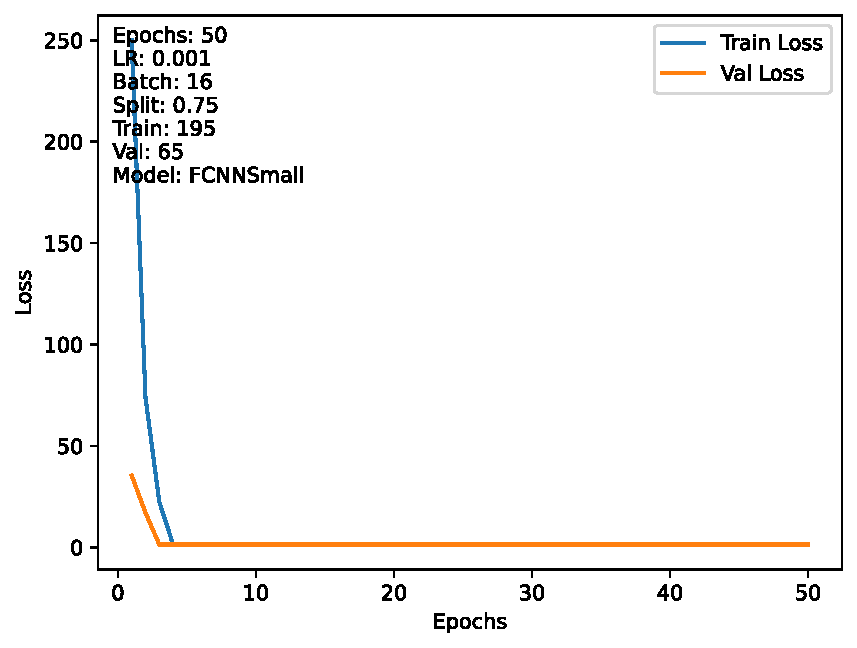
\includegraphics[width=\linewidth]{images/mhh_idana_num_classes_4_FCNNSmall_loss.pdf}
		\caption{FCNNSmall - Loss}
	\end{subfigure}
	\hfill
	\begin{subfigure}{0.3\textwidth}
		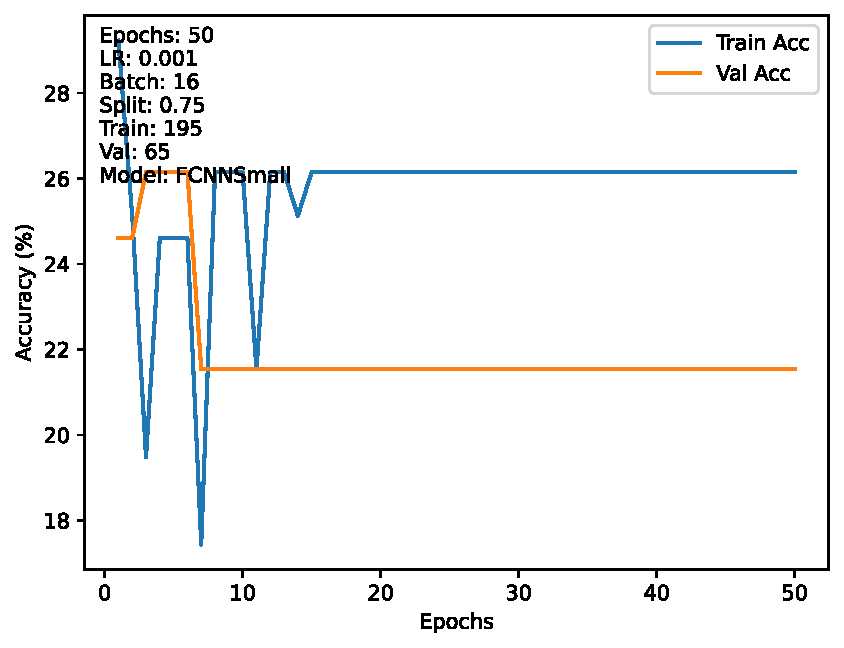
\includegraphics[width=\linewidth]{images/mhh_idana_num_classes_4_FCNNSmall_accuracy.pdf}
		\caption{FCNNSmall - Accuracy}
	\end{subfigure}
	\hfill
	\begin{subfigure}{0.3\textwidth}
		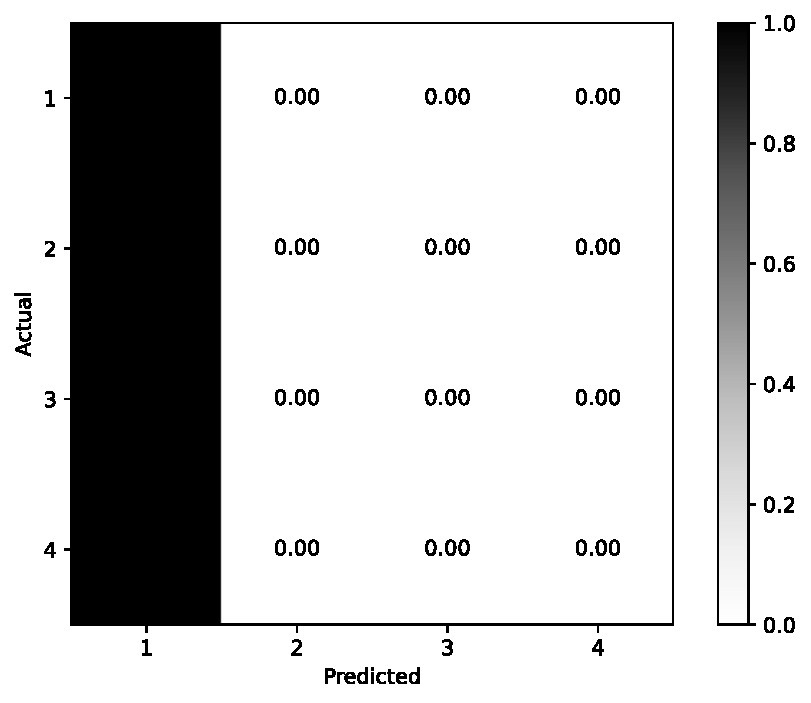
\includegraphics[width=\linewidth]{images/mhh_idana_num_classes_4_FCNNSmall_confusion_matrix.pdf}
		\caption{FCNNSmall - Confusion Matrix}
	\end{subfigure}
	
	\vspace{0.3cm}
	
	% ================= Row 3: Model 3 =================
	\begin{subfigure}{0.3\textwidth}
		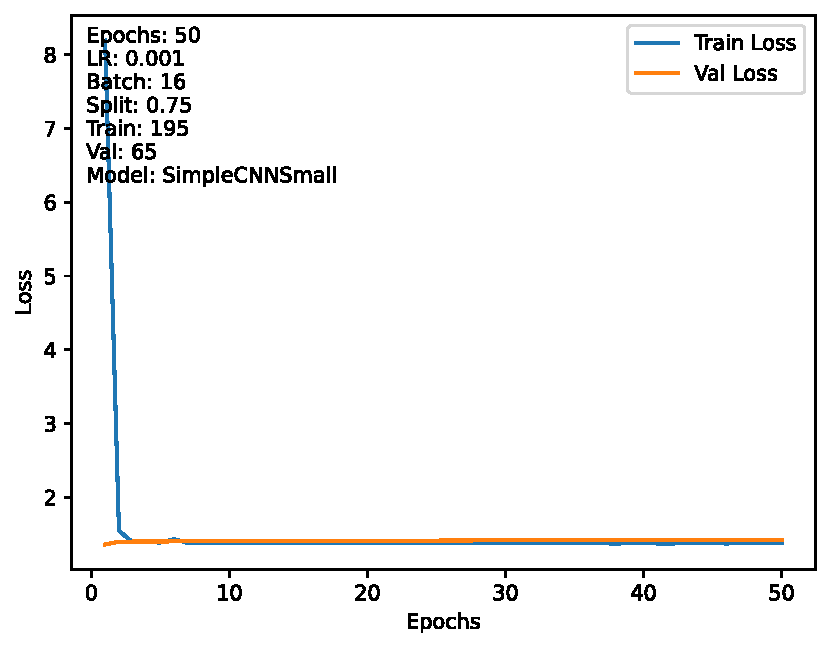
\includegraphics[width=\linewidth]{images/mhh_idana_num_classes_4_SimpleCNNSmall_loss.pdf}
		\caption{SimpleCNNSmall - Loss}
	\end{subfigure}
	\hfill
	\begin{subfigure}{0.3\textwidth}
		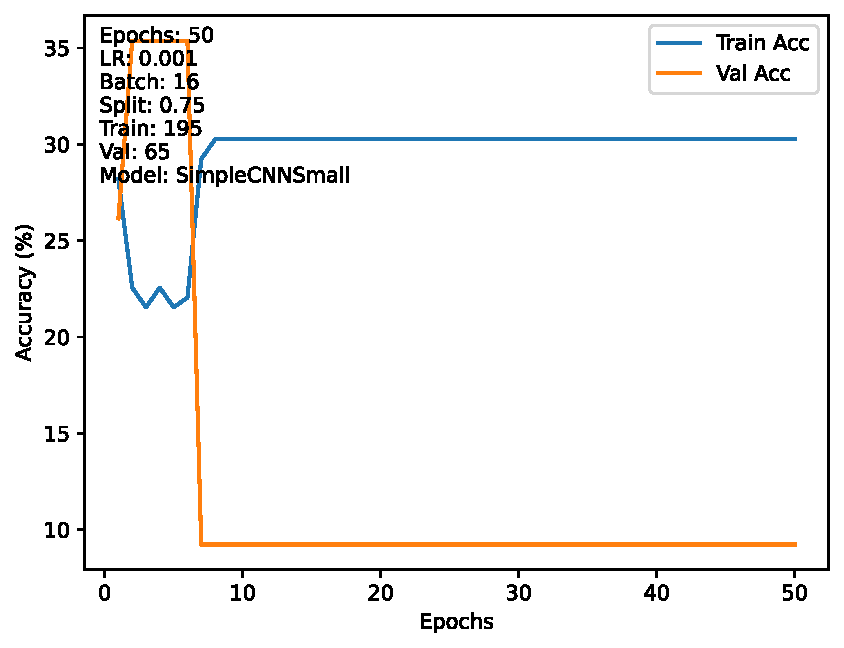
\includegraphics[width=\linewidth]{images/mhh_idana_num_classes_4_SimpleCNNSmall_accuracy.pdf}
		\caption{SimpleCNNSmall - Accuracy}
	\end{subfigure}
	\hfill
	\begin{subfigure}{0.3\textwidth}
		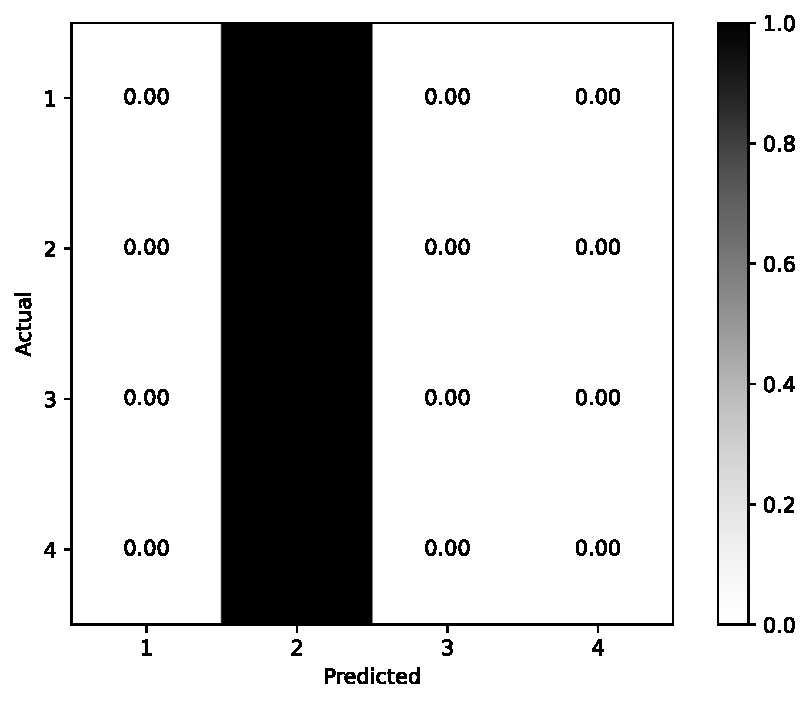
\includegraphics[width=\linewidth]{images/mhh_idana_num_classes_4_SimpleCNNSmall_confusion_matrix.pdf}
		\caption{SimpleCNNSmall - Confusion Matrix}
	\end{subfigure}
	
	\caption{Dataset 3: Model comparison (Loss, Accuracy, and Confusion Matrix) — MHH Idana dataset, 4 classes}
\end{figure}

\begin{figure}[H]
	\centering
	
	% ================= Row 1: Model 1 =================
	\begin{subfigure}{0.3\textwidth}
		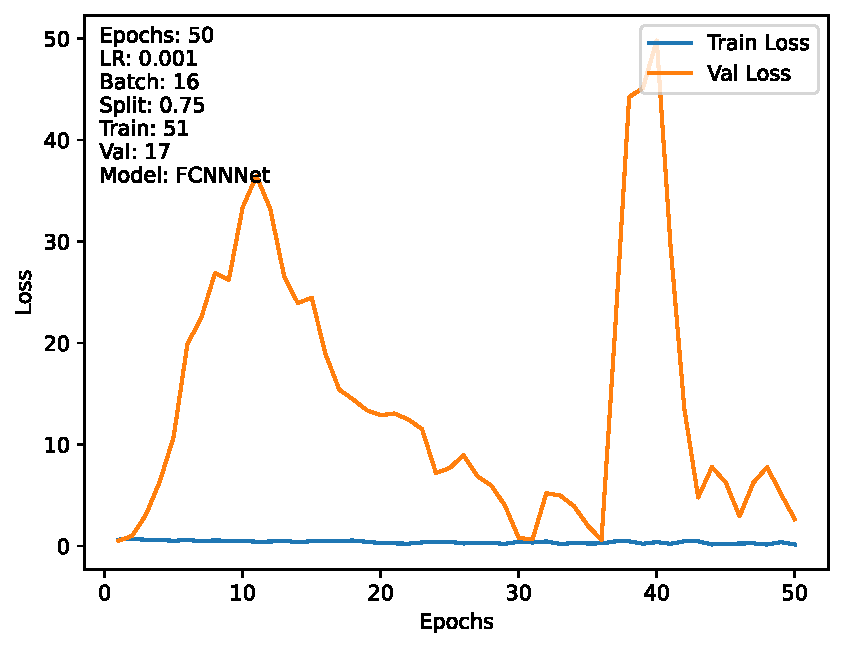
\includegraphics[width=\linewidth]{images/munich_num_classes_2_FCNNNet_loss.pdf}
		\caption{FCNNNet - Loss}
	\end{subfigure}
	\hfill
	\begin{subfigure}{0.3\textwidth}
		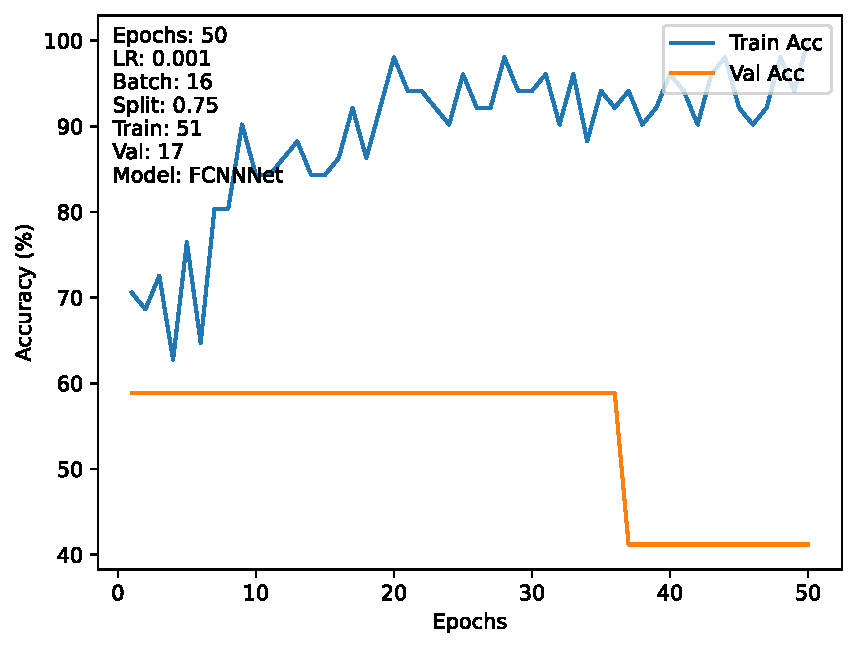
\includegraphics[width=\linewidth]{images/munich_num_classes_2_FCNNNet_accuracy.pdf}
		\caption{FCNNNet - Accuracy}
	\end{subfigure}
	\hfill
	\begin{subfigure}{0.3\textwidth}
		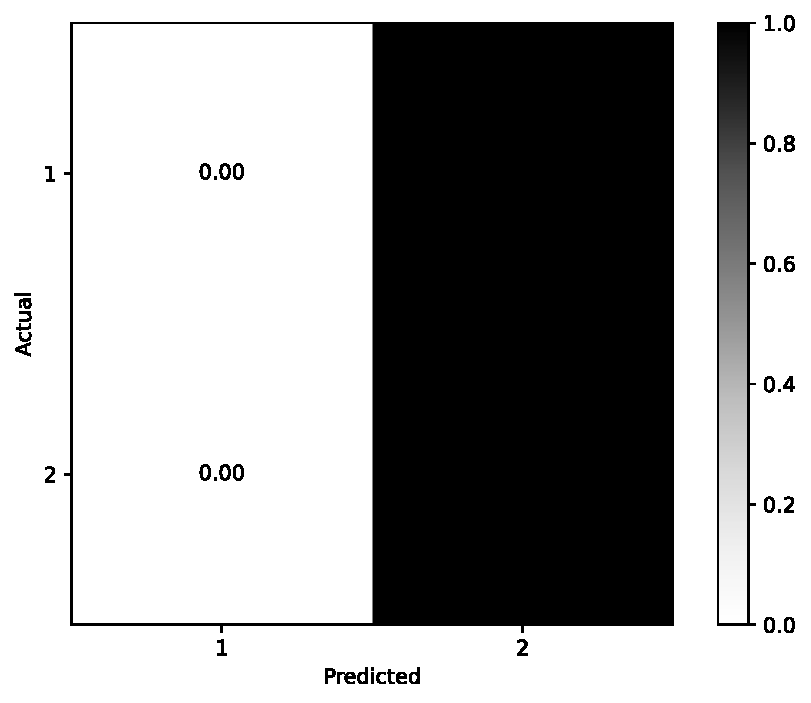
\includegraphics[width=\linewidth]{images/munich_num_classes_2_FCNNNet_confusion_matrix.pdf}
		\caption{FCNNNet - Confusion Matrix}
	\end{subfigure}
	
	\vspace{0.3cm}
	
	% ================= Row 2: Model 2 =================
	\begin{subfigure}{0.3\textwidth}
		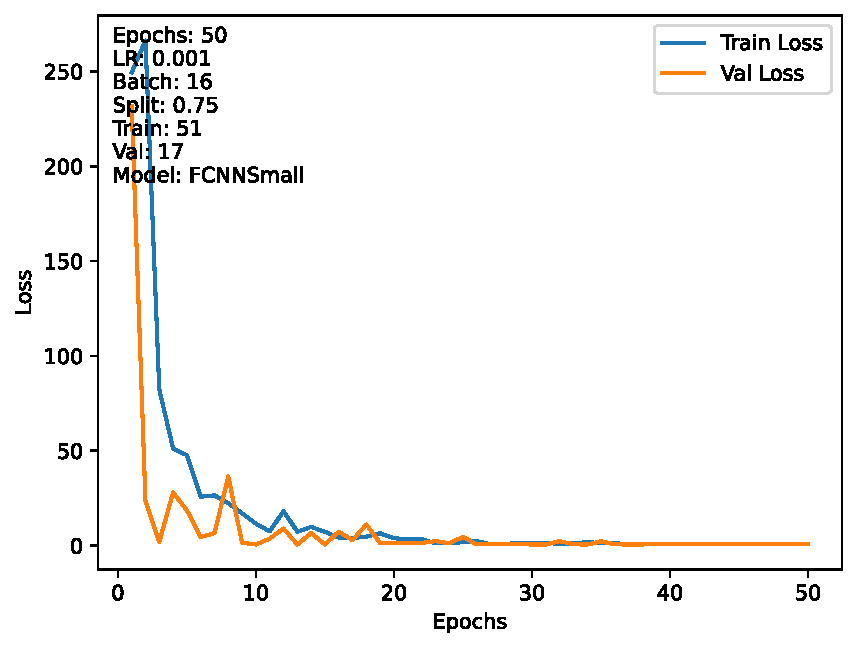
\includegraphics[width=\linewidth]{images/munich_num_classes_2_FCNNSmall_loss.pdf}
		\caption{FCNNSmall - Loss}
	\end{subfigure}
	\hfill
	\begin{subfigure}{0.3\textwidth}
		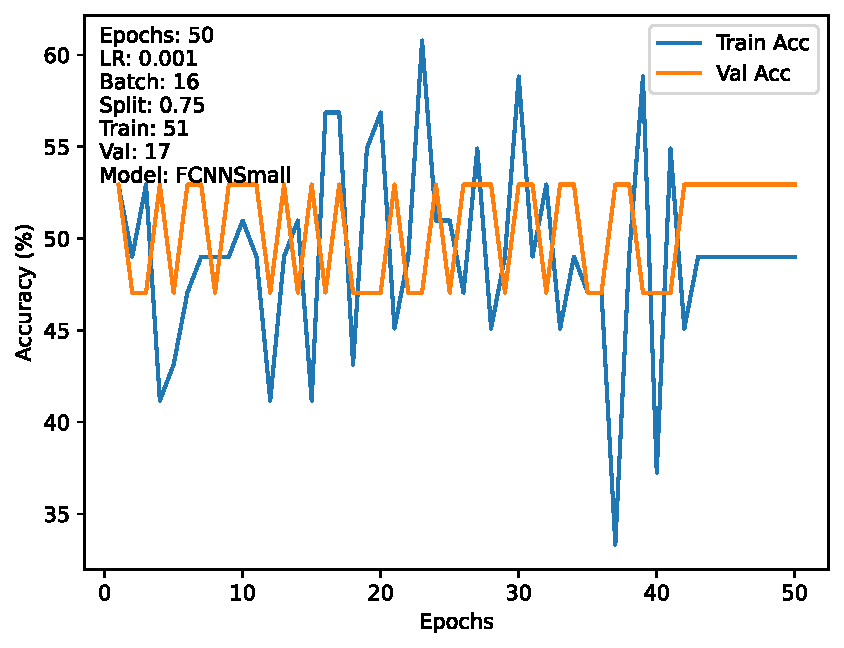
\includegraphics[width=\linewidth]{images/munich_num_classes_2_FCNNSmall_accuracy.pdf}
		\caption{FCNNSmall - Accuracy}
	\end{subfigure}
	\hfill
	\begin{subfigure}{0.3\textwidth}
		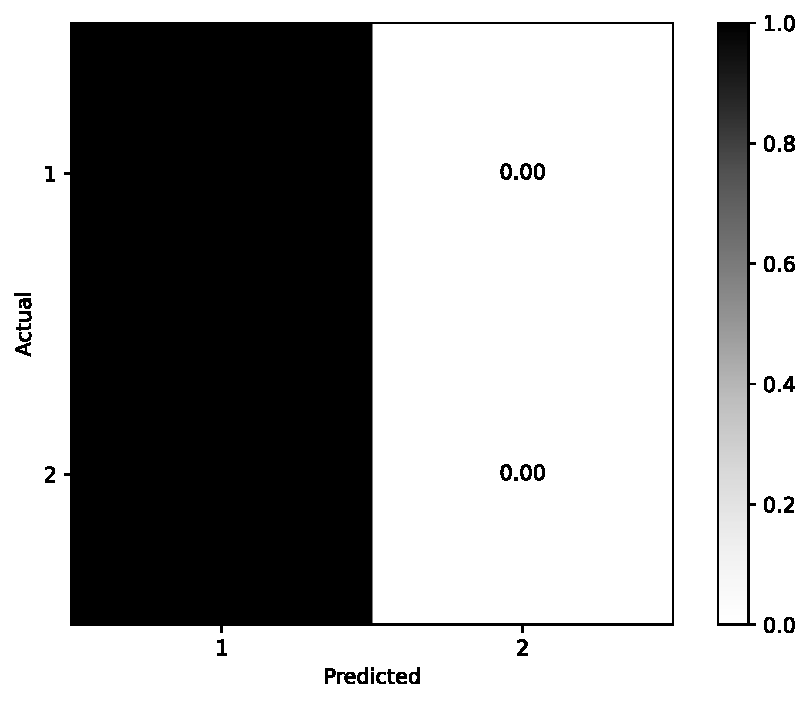
\includegraphics[width=\linewidth]{images/munich_num_classes_2_FCNNSmall_confusion_matrix.pdf}
		\caption{FCNNSmall - Confusion Matrix}
	\end{subfigure}
	
	\vspace{0.3cm}
	
	% ================= Row 3: Model 3 =================
	\begin{subfigure}{0.3\textwidth}
		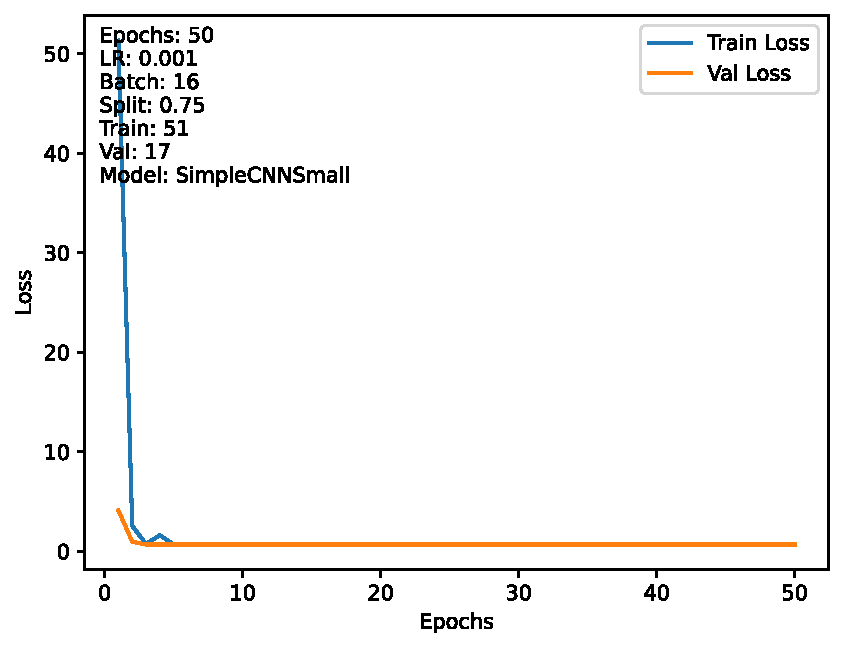
\includegraphics[width=\linewidth]{images/munich_num_classes_2_SimpleCNNSmall_loss.pdf}
		\caption{SimpleCNNSmall - Loss}
	\end{subfigure}
	\hfill
	\begin{subfigure}{0.3\textwidth}
		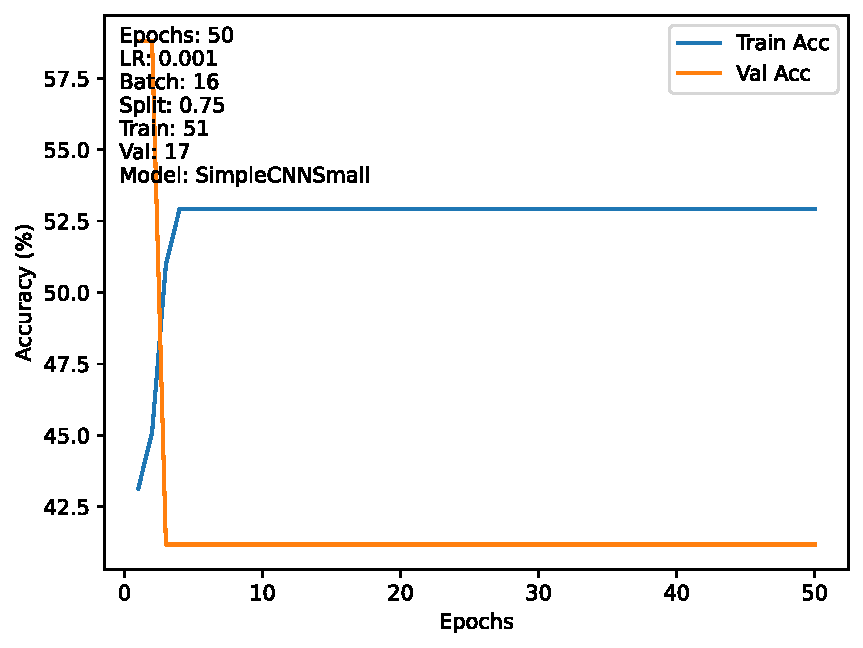
\includegraphics[width=\linewidth]{images/munich_num_classes_2_SimpleCNNSmall_accuracy.pdf}
		\caption{SimpleCNNSmall - Accuracy}
	\end{subfigure}
	\hfill
	\begin{subfigure}{0.3\textwidth}
		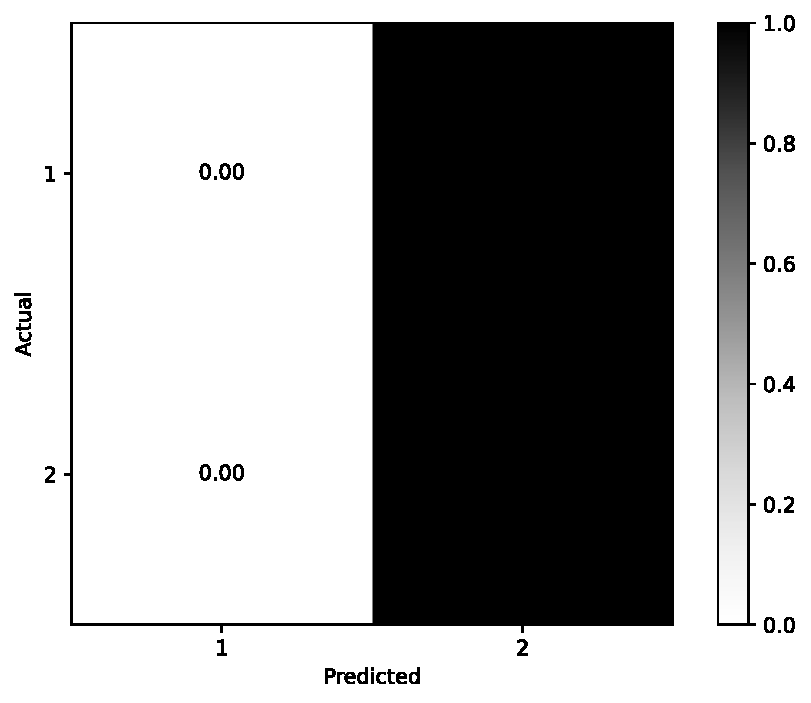
\includegraphics[width=\linewidth]{images/munich_num_classes_2_SimpleCNNSmall_confusion_matrix.pdf}
		\caption{SimpleCNNSmall - Confusion Matrix}
	\end{subfigure}
	
	\caption{Dataset 4: Model comparison (Loss, Accuracy, and Confusion Matrix) — Munich dataset, 2 classes}
\end{figure}

% -----------------------------
\chapter{Conclusion}
Summarize progress so far.

% -----------------------------
\chapter{Future Work}
\begin{itemize}
    \item Improve dataset quality
    \item Experiment with advanced models
    \item Collect more data
\end{itemize}

% -----------------------------
\chapter{References}
\bibliographystyle{plain}
\bibliography{references}

\begin{thebibliography}{9}
	
	\bibitem{litjens2017survey}
	G. Litjens et al., "A survey on deep learning in medical image analysis," \textit{Medical Image Analysis}, vol. 42, pp. 60–88, 2017.
	
	\bibitem{esteva2017dermatologist}
	A. Esteva et al., "Dermatologist-level classification of skin cancer with deep neural networks," \textit{Nature}, vol. 542, no. 7639, pp. 115–118, 2017.
	
	\bibitem{lecun2015deep}
	Y. LeCun, Y. Bengio, and G. Hinton, "Deep learning," \textit{Nature}, vol. 521, no. 7553, pp. 436–444, 2015.
	
	\bibitem{shen2017deep}
	D. Shen, G. Wu, and H.-I. Suk, "Deep learning in medical image analysis," \textit{Annual Review of Biomedical Engineering}, vol. 19, pp. 221–248, 2017.
	
	\bibitem{wester2020pain}
	L. Wester et al., "Pain drawings as a diagnostic tool for the differentiation between two pain-associated rare diseases (Ehlers-Danlos Syndrome, Guillain-Barré Syndrome)," 2020.
	
	\bibitem{emmert2018pain2d}
	D. Emmert et al., "A diagnostic support system based on pain drawings: binary and k-disease classification of EDS, GBS, FSHD, PROMM, and a control group with Pain2D," 2018.
	
\end{thebibliography}

\end{document}\\